

\documentclass{article}

\usepackage{amsmath}
\usepackage{graphicx}


\author{Qing Scholten, Wessel van Sommeren}
\title{Controlling a rabbit plaque}

\begin{document}

\maketitle
\newpage
\tableofcontents
\newpage

\section{Introduction}
In 1859 the First Fleet of settlers arrived in Australia, with them Thomas Austin. Thomas Austin took 13 European rabbits with him on his journey, so that once in Australia he could set them free so that he could hunt them for food. What Thomas Austin did not know was that these European rabbits did not have any natural predators or competition in australia. So by 1920 the small population of 13 rabbits had turned into a rabbit plaque, in 1920 there were an estimated 10 billion rabbits in australia.In this paper we will attempt to model the rabbit plaque of australia by exploring the question "What is the most effective way to control a rabbit plaque comparing Hunting, Introducing a predator and Introducing a Competitor 
\section{Base case}
For the base case we use the fact that a rabbit on average gets 4 - 8 babies per 60 days. So we take 6 on average that means one rabbit produces 0.1 rabbit per day. A rabbit in the wild live up to 9 nine years this means 0.000312109862672 rabbits die per day per rabbit. This means we get 
$$
\frac{dP(t)}{dt} = 0.1P(t)-0.000312109862672P(t)
$$

We take $P(0) = 13$ as starting population
\\

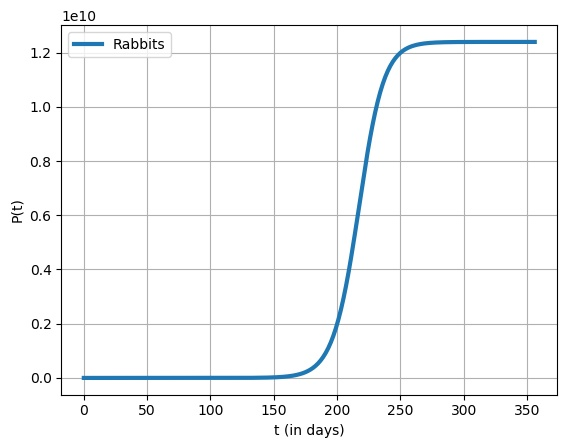
\includegraphics[scale=0.78]{Pictures/unr_rabbitts}
\\ 
As we can see from the graph de population of 13 rabbits grew to more than  $2.5\cdot10^{11}$ in just 250 days. This would continue to grow exponentially forever as the current model does not have a limiting factor. The limiting factor in our model is going to be food. As Australia has about 7 616 666 square kilometer land and 1 371 000 square kilometer of this land is desert, one finds that about 7 479 566 square kilometer is fertile land. This follows from the assumption that every land outside the deserts is able to grow grass, which is the vegetation that is used in the model. Known is that "the average annual total herbage production at Moorepark for the period 2005–9 was 14 087 kg DM/ ha, with an average grass growth of 50·3 kg DM/ha/day." A 1 hectare is equal to 0.01 square kilometer, the avarage annual total herbage production 140.87 kg $Dm/km^2$, so for Australia this is about 1 052 646 462 kg Dm. This means that the amount of grass, as grass has about 17 dry material, is about 6 197 920 367 kg grass for the whole of Australia. As rabbits eat around 1 cup of grass for 2 lbs of body weight, this would convert to about 0.25 kilo gram grass for a medium sized rabbit of 2 kilo gram. This means that Australia has enough grass to house 12 395 840 734 rabbits without running out of food.

Let $R$ be the reproduction number
$$
R = 0.1 - 0.000312109862672
$$
$$
\frac{dP(t)}{dt} = RP(t)(1-\frac{R}{12 395 840 734}P)
$$
\\
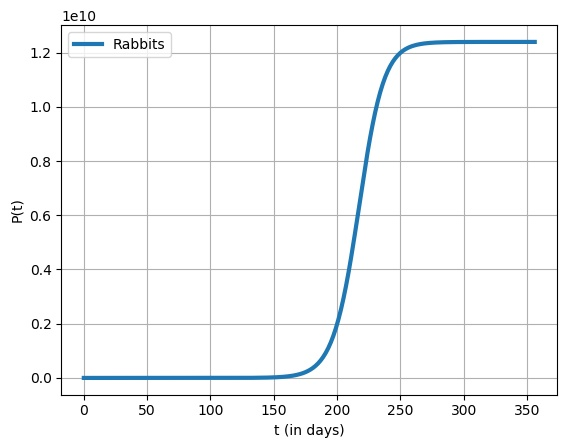
\includegraphics[scale=0.78]{Pictures/logis}
\end{document}
